\documentclass[12pt, letterpaper, parskip = full]{article}
\usepackage[mmddyyyy]{datetime}

\usepackage[utf8]{inputenc}
\usepackage{amsmath}
\usepackage{mathpazo}
\usepackage{eulervm}

\usepackage[margin=1in]{geometry}
\linespread{1.20}
\usepackage{enumerate}
\usepackage{enumitem}
\usepackage{listings}
\usepackage[T1]{fontenc}
\usepackage{amsfonts}
\usepackage{amssymb}
\usepackage{amsthm}
\usepackage{multirow,array}
\usepackage{graphicx}
\usepackage{physics}
\usepackage{bm}
\usepackage{tikz}
\usepackage{breqn}
\usepackage[longnamesfirst]{natbib}
\usepackage{comment}
\usepackage{setspace}
\usepackage{hyperref}

\graphicspath{{Images/}}

\newtheorem{theorem}{Theorem}
\newtheorem{corollary}{Corollary}
\newtheorem{lemma}{Lemma}
\newtheorem{definition}{Definition}
\newtheorem{axiom}{Axiom}
\newcommand{\e}{\mathrm{e}}
\newcommand{\Var}{\mathrm{Var}}
\newcommand{\Ex}[1]{\mathbb{E}\left[#1\right]}
\renewcommand{\Pr}[1]{\mathbb{P}(#1)}
\newcommand{\plim}{\mathrm{plim}}
\newcommand{\pc}[1]{\frac{\dot{#1}(t)}{#1(t)}}
\renewcommand\qedsymbol{$\blacksquare$}

\title{Homework 3}
\author{Alejandro Flores-Brown}

\begin{document}

  \maketitle

  \section{Problem 1}

  \subsection{Part A}

  Under the provided values, the income grid is
  \[   \begin{bmatrix}  0.277752 & 0.369224 & 0.490819 & 0.652458 & 0.86733  & 1.15296 & 1.53267 & 2.03741 & 2.70839 & 3.60033 \end{bmatrix}
 \]
 and the transition matrix is
 \tiny
 \begin{verbatim}
0.652258     0.312963     0.0341769    0.000599974  1.56892e-6   5.829e-10    2.9976e-14   0.0          0.0          0.0
0.168334     0.509838     0.292178     0.029183     0.000466515  1.10752e-6   3.7292e-10   1.73195e-14  0.0          0.0
0.0103624    0.176478     0.516406     0.271587     0.0248048    0.000361014  7.78001e-7   2.37403e-10  9.99201e-15  0.0
0.000123594  0.0123637    0.194068     0.520832     0.251348     0.0209867    0.00027804   5.43857e-7   1.50386e-10  5.77316e-15
2.61947e-7   0.000162566  0.0148169    0.212472     0.523058     0.231601     0.0176748    0.000213113  3.78324e-7   9.47967e-11
9.47967e-11  3.78324e-7   0.000213113  0.0176748    0.231601     0.523058     0.212472     0.0148169    0.000162566  2.61947e-7
5.73782e-15  1.50386e-10  5.43857e-7   0.00027804   0.0209867    0.251348     0.520832     0.194068     0.0123637    0.000123594
5.74006e-20  1.00047e-14  2.37403e-10  7.78001e-7   0.000361014  0.0248048    0.271587     0.516406     0.176478     0.0103624
9.42111e-26  1.10056e-19  1.73578e-14  3.7292e-10   1.10752e-6   0.000466515  0.029183     0.292178     0.509838     0.168334
2.52461e-32  1.98689e-25  2.0996e-19   2.99656e-14  5.829e-10    1.56892e-6   0.000599974  0.0341769    0.312963     0.652258
 \end{verbatim}
\normalsize
 I will note that there is an error in the code for the Tauchen process which produces the same transition matrix regardless of inputs (conditional on the size). I have yet to figure out why this is in spite of several days of trying. The rest of the code appears to be error-free.

 \subsection{Part B}

  The next period's distribution is
  \small
  \[  \begin{bmatrix} 0.0831079 & 0.101181 & 0.105186 & 0.105263 & 0.105263 & 0.105263 & 0.105263 & 0.105186 & 0.101181 & 0.0831079 \end{bmatrix} \]
  \normalsize

  \subsection{Part C}

  The stationary distribution is computed by matrix exponentiation (to \(n=1000\), which appears to ensure convergence). It is given by
  \tiny
  \[ \begin{bmatrix}  0.0322302 & 0.0603013 & 0.100323 & 0.140633 & 0.166513 & 0.166513 & 0.140633 & 0.100323 & 0.0603013 & 0.0322302 \end{bmatrix} \]
  \normalsize

  \subsection{Parts D and E}


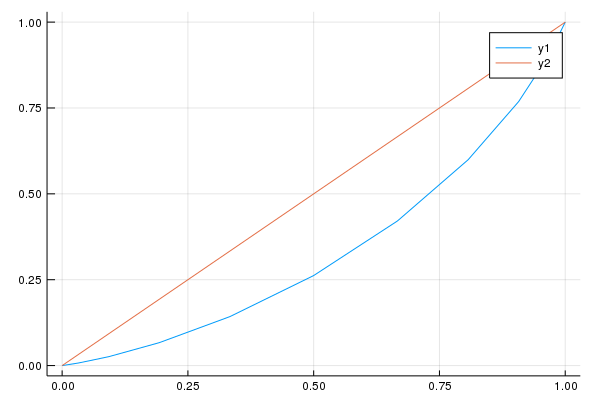
\includegraphics[scale=0.3]{p1_1}
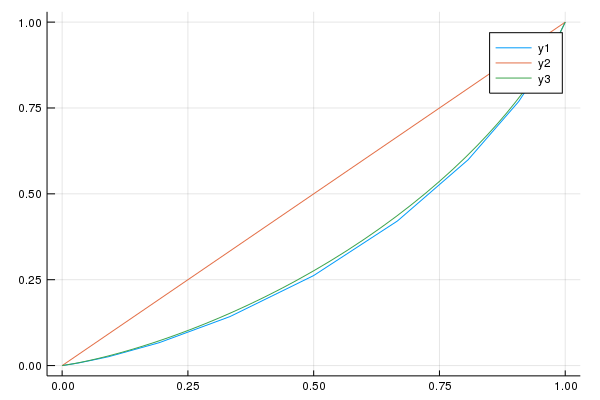
\includegraphics[scale=0.3]{p1_2}


  \begin{table}[]
\begin{tabular}{|lllllll|}
\hline
                         & Variance & Coefficient & Gini  & Mean/Median & 90/50 & 50/10 \\ \cline{2-7}
\multicolumn{1}{|l|}{10} & 0.385    & 0.635       & 0.335 & 1.393       & 2.349 & 1.767 \\
\multicolumn{1}{|l|}{50} & 0.342    & 0.601       & 0.320 & 1.153       & 2.079 & 2.191 \\ \hline
\end{tabular}
\end{table}

  \section{Problem 2}

  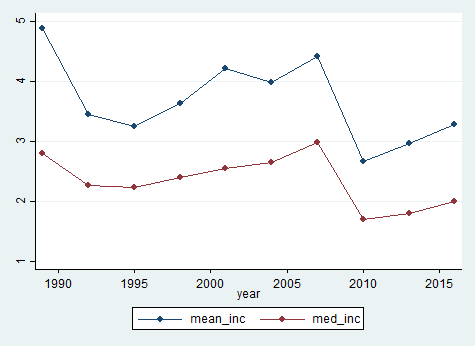
\includegraphics[scale=0.3]{inc.png}
  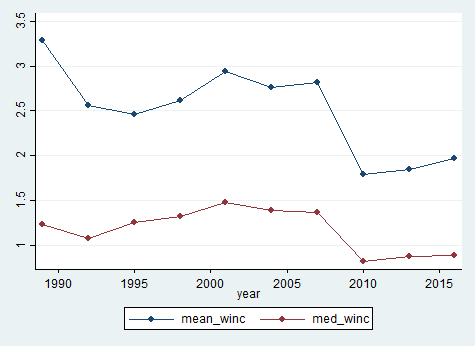
\includegraphics[scale=0.3]{winc.png}

  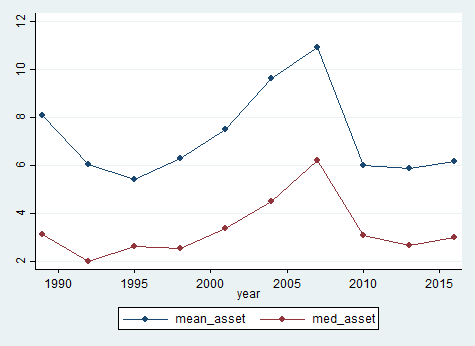
\includegraphics[scale=0.3]{asset.png}
  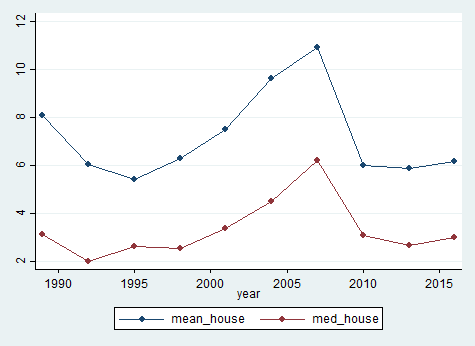
\includegraphics[scale=0.3]{house.png}

  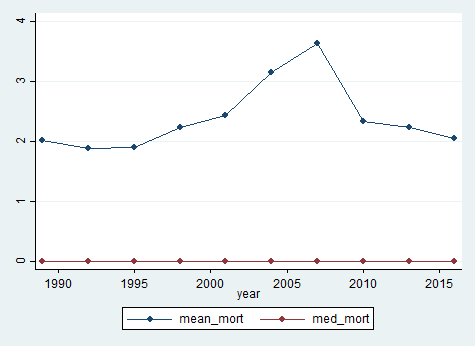
\includegraphics[scale=0.3]{mort.png}
  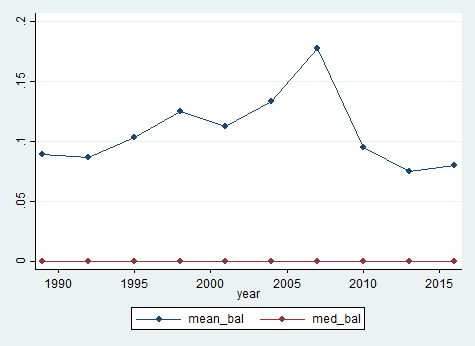
\includegraphics[scale=0.3]{bal.png}

  \section{Problem 3}

  I have computations for these problems, but with the error remaining in the Tauchen process, there is no point in showing them because my work shows no evolution. The code I used is attached.

  \appendix

Julia Code

\begin{lstlisting}[breaklines]
using Distributions, LinearAlgebra, Plots

#fundamental parameters
const rho1 = 0.95
const sigma1 = 0.20
const mu1 = 0

#grid parameters
lambda1 = 2
m1 = 10
m2 = 50

function Tauchen(lambda::Number, m::Number, rho::Number, sigma::Number, mu::Number)
    #discretize AR(1) process
    local z1 = mu - lambda * sigma * (1-rho^2)^(-0.5)
    local step = -2*z1*(m-1)^(-1)
    local zm = z1 + (m-1)*step
    local AR1 = collect(range(z1, length=m, stop=zm))

    #Compute transition matrix
    local TransMat = zeros(m,m)
    local quant

    for j=1:m
        for k=1:m

            quant=0
            if k==1
                quant = cdf(Normal(), ((AR1[k] + 0.5*step - rho*AR1[j])/sigma) )
            elseif k==m
                quant = 1 - cdf(Normal(), ((AR1[k] - 0.5*step - rho*AR1[j])/sigma) )
            else
                quant = cdf(Normal(), ((AR1[k] + 0.5*step - rho*AR1[j])/sigma) ) - cdf(Normal(), ((AR1[k] - 0.5*step - rho*AR1[j])/sigma) )
            end
            TransMat[j,k] = quant
        end
    end

    return AR1, TransMat
end

function staDist(M::Array{Float64,2})
    local n = size(M)[1]
    local Vold = transpose(collect(range(1/n, length=n, stop=1/n)))
    local Vnew
    for i=1:10000
        Vnew = zeros(n)
        Vnew = Vold * M
        Vold = zeros(n)
        Vold = Vnew
    end
    #create return value of type Array and not type Transpose
    local Vret = zeros(n)
    for i=1:n
        Vret[i] = Vnew[i]
    end
    return Vret
end

function trueIncome(v::Array{Float64,1})
    local temp = zeros(length(v))
    for i=1:length(v)
        temp[i] = exp(v[i])
    end
    return temp
end

function tmat(A::Array{Float64,2})
    local B = zeros(size(A'))
    for i=1:size(B)[1]
        for j=1:size(B)[2]
            B[i,j] = A[j,i]
        end
    end
    return B
end

function compStats(z::Array{Float64,1}, p::Array{Float64,1})
    local y = trueIncome(z)
    local z2 = z.^2
    local y2 = y.^2

    #Variance
    local sigmaz2 = dot(p,z2) - dot(p,z)^2
    #Coefficient of Variation
    local sigmay2 = dot(p,y2) - dot(p,y)^2
    local coeff = sqrt(sigmay2)/dot(p,y)

    #percentiles
    local medfinder = findfirst(x -> x > 0.5, cumsum(p))
    local tenfinder = findfirst(x -> x > 0.1, cumsum(p))
    local ninfinder = findfirst(x -> x > 0.9, cumsum(p))
    local med = y[medfinder]
    local ten = y[tenfinder]
    local nin = y[ninfinder]

    #mean/median
    local mm = dot(p,y)/med
    #90/50
    local nm = nin/med
    #50/10
    local mt = med/ten

    #Gini coefficient
    local g = zeros(length(y),length(y))
    for i=1:length(y)
        for j=1:length(y)
            g[i,j] = abs(y[i] - y[j]) *p[i] * p[j]
        end
    end
    local Gini = (2*dot(y,p))^(-1)*sum(g)

    #Prepare simulated Lorenz curve data
    local F = [0; cumsum(p)]
    local Ltemp = [0; cumsum(y.*p)]
    local L = Ltemp/Ltemp[length(Ltemp)]
    local lp = collect(range(0,length=length(L),stop=1))

    return sigmaz2, coeff, Gini, mm, nm, mt, F, L, lp

end

function compDists(n::Number, lambda::Number, m::Number, rho::Number, sigma::Number, mu::Number)
    sigmasigma = collect(range(sigma, length=n, step=0.005))
    #local zs = Array{Array{Float64,1}, n}
    #local ps = Array{Array{Float64,2}, n}

    #local zs = fill(zeros(n), 1, n)
    local z = Tauchen(lambda, m, rho, sigmasigma[1], mu)[1]
    local ps = fill(zeros(n,n), 1, n)
    for i=1:n
        #zs[i] = Tauchen(lambda, m, rho, sigmasigma[i], mu)[1]
        ps[i] = Tauchen(lambda, m, rho, sigmasigma[i], mu)[2]
    end

    #local dists = Array{Array{Float64,1}, n}
    local dist = staDist(ps[1])
    #for i=1:n
    #   dists[i] = staDist(ps[i])
    #end

    return z, ps, dist
end

function multMats(ps = Array{Array{Float64,2}}, z = Array{Float64,1})
    n = length(z)
    m = length(ps)
    local zold = z
    local znew
    #local zs = fill(zeros(n), 1, n)
    local zlist = fill(zeros(n), 1, m)
    zlist[1] = z

    #transpose matrices
    local plist = fill(zeros(n,n), 1, n)
    for i=1:m
        for j=1:n
            for k=1:n
                plist[i][j,k] = ps[i][k,j]
            end
        end
    end

    #multiply once by every transition matrix after the first (1989)
    for i=2:m
        znew = zeros(n)
        znew = plist[i] * zold
        zlist[i] = znew
        zold = zeros(n)
        zold = znew
    end

    #create return values of type Array and not type Transpose
    #local Vret = zeros(n)
    #for i=1:n
    #    Vret[i] = Vnew[i]
    #end
    return zlist
end

#Problem 1
IP1 = Tauchen(lambda1, m1, rho1, sigma1, mu1)
z1 = IP1[1]
y1 = trueIncome(z1)
M1 = IP1[2]

V1 = collect(range(0.1, length=10, stop=0.1))
V2 = V1'*IP1[2]

#Part C

#compute matrix exponential
matinf1 = M1^1000
#get first row (any will do; all are equivalent)
stad1 = matinf1[1,:]
#check against another way of finding π
Vf1 = staDist(M1)

#Part D
stats1 = compStats(z1,stad1)

#Part E
IP2 = Tauchen(lambda1, m2, rho1, sigma1, mu1)
z2 = IP2[1]
y2 = trueIncome(z2)
M2 = IP2[2]
Vf2 = staDist(IP2[2])
matinf2 = M2^1000
#get first row (any will do; all are equivalent)
stad2 = matinf2[1,:]
stats2 = compStats(z2,stad2)

lorenzes = plot(stats1[7], stats1[8])
plot!(lorenzes, stats1[9], stats1[9])
savefig("p1_1")
plot!(lorenzes, stats2[7], stats2[8])
savefig("p1_2")

#Problem 3

const ncomps = 2016 - 1989 + 1
seqDists = compDists(ncomps, lambda1, m2, rho1, sigma1, mu1)

grid = trueIncome(seqDists[1])
mats = seqDists[2]
dist = seqDists[3]

evp = multMats(mats, dist)

#=
    #Gini coefficient
    local g = zeros(length(y),length(y))
    for i=1:length(y)
        for j=1:length(y)
            g[i,j] = abs(y[i] - y[j]) *p[i] * p[j]
        end
    end
    local Gini = (2*dot(y,p))^(-1)*sum(g)
=#

meanIncs = zeros(ncomps)
medIncs = zeros(ncomps)
cumIncs = fill(zeros(length(grid)), 1, ncomps)
Ginis = zeros(ncomps)

for i=1:ncomps
    meanIncs[i] = dot(evp[i], grid)
    cumIncs[i] = cumsum(evp[i])
    medIncs[i] = grid[findfirst(x -> x > 0.5, cumsum(evp[i]))]
    local g = zeros(length(grid), length(grid))
    for j=1:length(grid)
        for k=1:length(grid)
            g[j,k] = abs(grid[j] - grid[k]) * evp[i][j] * evp[i][k]
        end
    end
    Ginis[i] = (2*dot(grid,evp[i]))^(-1) * sum(g)
end

times = collect(range(1989, step=1, stop=2016))
plot([times meanIncs])
savefig("p2_1")
plot([times Ginis])
savefig("p2_2")

\end{lstlisting}

Stata Code

\begin{lstlisting}[breaklines]
clear

cd "C:\Users\Alejandro\Box Sync\S19\Quant Macro\Homework\Homework 3\extracts"
use rscfp2016.dta

keep wgt income wageinc houses asset NH_MORT ccbal

egen sumwgt = sum(wgt)

gen wgt_alt = wgt/sumwgt
gen alt_inc = wgt_alt*income
gen alt_winc = wgt_alt*wageinc
gen alt_house = wgt_alt*houses
gen alt_asset = wgt_alt*houses
gen alt_mort = wgt_alt*NH_MORT
gen alt_bal = wgt_alt*ccbal
gen year = 2016

egen mean_inc = mean(alt_inc)
egen med_inc = median(alt_inc)

egen mean_winc = mean(alt_winc)
egen med_winc = median(alt_winc)

egen mean_house = mean(alt_house)
egen med_house = median(alt_house)

egen mean_asset = mean(alt_asset)
egen med_asset = median(alt_asset)

egen mean_mort = mean(alt_mort)
egen med_mort = median(alt_mort)

egen mean_bal = mean(alt_bal)
egen med_bal = median(alt_bal)

save 2016.dta, replace
clear

use rscfp2013.dta

keep wgt income wageinc houses asset NH_MORT ccbal

egen sumwgt = sum(wgt)

gen wgt_alt = wgt/sumwgt
gen alt_inc = wgt_alt*income
gen alt_winc = wgt_alt*wageinc
gen alt_house = wgt_alt*houses
gen alt_asset = wgt_alt*houses
gen alt_mort = wgt_alt*NH_MORT
gen alt_bal = wgt_alt*ccbal
gen year = 2013

egen mean_inc = mean(alt_inc)
egen med_inc = median(alt_inc)

egen mean_winc = mean(alt_winc)
egen med_winc = median(alt_winc)

egen mean_house = mean(alt_house)
egen med_house = median(alt_house)

egen mean_asset = mean(alt_asset)
egen med_asset = median(alt_asset)

egen mean_mort = mean(alt_mort)
egen med_mort = median(alt_mort)

egen mean_bal = mean(alt_bal)
egen med_bal = median(alt_bal)
save 2013.dta, replace
clear

use rscfp2010.dta

keep wgt income wageinc houses asset NH_MORT ccbal

egen sumwgt = sum(wgt)

gen wgt_alt = wgt/sumwgt
gen alt_inc = wgt_alt*income
gen alt_winc = wgt_alt*wageinc
gen alt_house = wgt_alt*houses
gen alt_asset = wgt_alt*houses
gen alt_mort = wgt_alt*NH_MORT
gen alt_bal = wgt_alt*ccbal
gen year = 2010

egen mean_inc = mean(alt_inc)
egen med_inc = median(alt_inc)

egen mean_winc = mean(alt_winc)
egen med_winc = median(alt_winc)

egen mean_house = mean(alt_house)
egen med_house = median(alt_house)

egen mean_asset = mean(alt_asset)
egen med_asset = median(alt_asset)

egen mean_mort = mean(alt_mort)
egen med_mort = median(alt_mort)

egen mean_bal = mean(alt_bal)
egen med_bal = median(alt_bal)
save 2010.dta, replace
clear

use rscfp2007.dta

keep wgt income wageinc houses asset NH_MORT ccbal

egen sumwgt = sum(wgt)

gen wgt_alt = wgt/sumwgt
gen alt_inc = wgt_alt*income
gen alt_winc = wgt_alt*wageinc
gen alt_house = wgt_alt*houses
gen alt_asset = wgt_alt*houses
gen alt_mort = wgt_alt*NH_MORT
gen alt_bal = wgt_alt*ccbal
gen year = 2007

egen mean_inc = mean(alt_inc)
egen med_inc = median(alt_inc)

egen mean_winc = mean(alt_winc)
egen med_winc = median(alt_winc)

egen mean_house = mean(alt_house)
egen med_house = median(alt_house)

egen mean_asset = mean(alt_asset)
egen med_asset = median(alt_asset)

egen mean_mort = mean(alt_mort)
egen med_mort = median(alt_mort)

egen mean_bal = mean(alt_bal)
egen med_bal = median(alt_bal)
save 2007.dta, replace
clear

use rscfp2004.dta

keep wgt income wageinc houses asset NH_MORT ccbal

egen sumwgt = sum(wgt)

gen wgt_alt = wgt/sumwgt
gen alt_inc = wgt_alt*income
gen alt_winc = wgt_alt*wageinc
gen alt_house = wgt_alt*houses
gen alt_asset = wgt_alt*houses
gen alt_mort = wgt_alt*NH_MORT
gen alt_bal = wgt_alt*ccbal
gen year = 2004

egen mean_inc = mean(alt_inc)
egen med_inc = median(alt_inc)

egen mean_winc = mean(alt_winc)
egen med_winc = median(alt_winc)

egen mean_house = mean(alt_house)
egen med_house = median(alt_house)

egen mean_asset = mean(alt_asset)
egen med_asset = median(alt_asset)

egen mean_mort = mean(alt_mort)
egen med_mort = median(alt_mort)

egen mean_bal = mean(alt_bal)
egen med_bal = median(alt_bal)
save 2004.dta, replace
clear

use rscfp2001.dta

keep wgt income wageinc houses asset NH_MORT ccbal

egen sumwgt = sum(wgt)

gen wgt_alt = wgt/sumwgt
gen alt_inc = wgt_alt*income
gen alt_winc = wgt_alt*wageinc
gen alt_house = wgt_alt*houses
gen alt_asset = wgt_alt*houses
gen alt_mort = wgt_alt*NH_MORT
gen alt_bal = wgt_alt*ccbal
gen year = 2001

egen mean_inc = mean(alt_inc)
egen med_inc = median(alt_inc)

egen mean_winc = mean(alt_winc)
egen med_winc = median(alt_winc)

egen mean_house = mean(alt_house)
egen med_house = median(alt_house)

egen mean_asset = mean(alt_asset)
egen med_asset = median(alt_asset)

egen mean_mort = mean(alt_mort)
egen med_mort = median(alt_mort)

egen mean_bal = mean(alt_bal)
egen med_bal = median(alt_bal)
save 2001.dta, replace
clear

use rscfp1998.dta

keep wgt income wageinc houses asset NH_MORT ccbal

egen sumwgt = sum(wgt)

gen wgt_alt = wgt/sumwgt
gen alt_inc = wgt_alt*income
gen alt_winc = wgt_alt*wageinc
gen alt_house = wgt_alt*houses
gen alt_asset = wgt_alt*houses
gen alt_mort = wgt_alt*NH_MORT
gen alt_bal = wgt_alt*ccbal
gen year = 1998

egen mean_inc = mean(alt_inc)
egen med_inc = median(alt_inc)

egen mean_winc = mean(alt_winc)
egen med_winc = median(alt_winc)

egen mean_house = mean(alt_house)
egen med_house = median(alt_house)

egen mean_asset = mean(alt_asset)
egen med_asset = median(alt_asset)

egen mean_mort = mean(alt_mort)
egen med_mort = median(alt_mort)

egen mean_bal = mean(alt_bal)
egen med_bal = median(alt_bal)
save 1998.dta, replace
clear

use rscfp1995.dta


keep wgt income wageinc houses asset NH_MORT ccbal

egen sumwgt = sum(wgt)

gen wgt_alt = wgt/sumwgt
gen alt_inc = wgt_alt*income
gen alt_winc = wgt_alt*wageinc
gen alt_house = wgt_alt*houses
gen alt_asset = wgt_alt*houses
gen alt_mort = wgt_alt*NH_MORT
gen alt_bal = wgt_alt*ccbal
gen year = 1995

egen mean_inc = mean(alt_inc)
egen med_inc = median(alt_inc)

egen mean_winc = mean(alt_winc)
egen med_winc = median(alt_winc)

egen mean_house = mean(alt_house)
egen med_house = median(alt_house)

egen mean_asset = mean(alt_asset)
egen med_asset = median(alt_asset)

egen mean_mort = mean(alt_mort)
egen med_mort = median(alt_mort)

egen mean_bal = mean(alt_bal)
egen med_bal = median(alt_bal)
save 1995.dta, replace
clear

use rscfp1992.dta

keep wgt income wageinc houses asset NH_MORT ccbal

egen sumwgt = sum(wgt)

gen wgt_alt = wgt/sumwgt
gen alt_inc = wgt_alt*income
gen alt_winc = wgt_alt*wageinc
gen alt_house = wgt_alt*houses
gen alt_asset = wgt_alt*houses
gen alt_mort = wgt_alt*NH_MORT
gen alt_bal = wgt_alt*ccbal
gen year = 1992

egen mean_inc = mean(alt_inc)
egen med_inc = median(alt_inc)

egen mean_winc = mean(alt_winc)
egen med_winc = median(alt_winc)

egen mean_house = mean(alt_house)
egen med_house = median(alt_house)

egen mean_asset = mean(alt_asset)
egen med_asset = median(alt_asset)

egen mean_mort = mean(alt_mort)
egen med_mort = median(alt_mort)

egen mean_bal = mean(alt_bal)
egen med_bal = median(alt_bal)
save 1992.dta, replace
clear

use rscfp1989.dta

keep wgt income wageinc houses asset NH_MORT ccbal

egen sumwgt = sum(wgt)

gen wgt_alt = wgt/sumwgt
gen alt_inc = wgt_alt*income
gen alt_winc = wgt_alt*wageinc
gen alt_house = wgt_alt*houses
gen alt_asset = wgt_alt*houses
gen alt_mort = wgt_alt*NH_MORT
gen alt_bal = wgt_alt*ccbal
gen year = 1989

egen mean_inc = mean(alt_inc)
egen med_inc = median(alt_inc)

egen mean_winc = mean(alt_winc)
egen med_winc = median(alt_winc)

egen mean_house = mean(alt_house)
egen med_house = median(alt_house)

egen mean_asset = mean(alt_asset)
egen med_asset = median(alt_asset)

egen mean_mort = mean(alt_mort)
egen med_mort = median(alt_mort)

egen mean_bal = mean(alt_bal)
egen med_bal = median(alt_bal)
save 1989.dta, replace

clear

use 2016.dta
append using 2013.dta
append using 2010.dta
append using 2007.dta
append using 2004.dta
append using 2001.dta
append using 1998.dta
append using 1995.dta
append using 1992.dta
append using 1989.dta
save scf.dta, replace

twoway connected mean_inc med_inc year
graph export inc.png, replace
twoway connected mean_winc med_winc year
graph export winc.png, replace
twoway connected mean_house med_house year
graph export house.png, replace
twoway connected mean_asset med_asset year
graph export asset.png, replace
twoway connected mean_mort med_mort year
graph export mort.png, replace
twoway connected mean_bal med_bal year
graph export bal.png, replace
\end{lstlisting}


\end{document}
